\chapter{Methodology for extracting and filtering logical dependencies}
\label{extraction}

\section{Overview of the approach}
\label{sec:overview_approach}

\hspace{4em}This chapter investigates the process of extracting and refining logical dependencies. The process is organized into three steps: collecting data, extracting dependencies, and applying filters.

A set of 27 open-source projects were used to perform the investigations. These projects have different sizes, complexities, and programming languages (Java and C\#). Section \ref{subsec:data_sets_used} provides an overview of the systems used.

The extraction process targets two types of dependencies:\\
- \textit{Structural dependencies} are obtained by analyzing the static structure of the source code. Using the \textit{srcML} tool, source code files are converted into an XML format to extract relationships between entities. \\
- \textit{Logical dependencies} are derived from the version control history. \\

After extraction, filtering techniques are applied to refine the logical dependencies:\\
- \textit{Commit size filtering} removes co-changing pairs from large commits, such as branch merges or formatting updates.\\
- \textit{Support filtering} ensures co-changing pairs occur a minimum number of times.\\
- \textit{Strength filtering} uses metrics like support, confidence, and a system factor to identify pairs with stronger relationships, scaling the results to the reality of the system.

Each filtering step helps reduce the number of co-changing pairs while keeping meaningful dependencies. Figure \ref{fig:figworkflow} shows the workflow of the tool, which handles data collection, dependency extraction, and filtering. 



\section{Data collection}
\label{sec:data_collection}


\subsection{Data set used}
\label{subsec:data_sets_used}

\hspace{4em}To investigate logical dependencies extraction and filtering techniques and their interplay with structural dependencies, 27 open-source projects from GitHub\footnote{http://github.com/} were selected. Table \ref{table:1} provides an overview of all the software systems analyzed. The columns in the table represent the following information:

\hspace{-4em}- \textit{ID}: A unique identifier assigned to each project. \\
- \textit{Project name}: The name of the project as it appears on GitHub. \\
- \textit{Number of entities}: The total number of entities (classes and interfaces) extracted from the source code. \\
- \textit{Number of commits}: The total number of commits analyzed from the active branch (main/master) of each project. \\
- \textit{Type}: The programming language used in the development of the project.


This selection includes projects implemented in two programming languages: Java and C\#. The systems vary in size and complexity. From a structural perspective, the smallest project is \textit{shipkit}, which contains only 639 entities, while the largest is \textit{EntityFrameworkCore}, with 50,179 entities.

Regarding commit history, \textit{shipkit} is again the smallest, with 1,563 commits analyzed, while \textit{aeron} is the largest, with 5,977 commits. This selection of projects allows a better investigation of how filtering techniques affect systems of different sizes and commit histories.


\begin{table}[!h]
\renewcommand{\arraystretch}{1}
\caption{Summary of open source projects used for logical dependencies extraction and filtering.}
\label{table:1}
\centering
\scalebox{0.9}{
\begin{tabular}{|c|c|c|c|c|c|}
\hline
   ID  & Project name   & Number of & Number of& Type\\
     &     & entites & commits & \\
\hline
1	&	bluecove	&	2685	&	894	&	Java	\\
2	&	aima-java	&	5232	&	1006	&	Java	\\
3	&	powermock	&	2801	&	949	&	Java	\\
4	&	restfb	&	3350	&	1391	&	Java	\\
5	&	rxjava	&	21097	&	4398	&	Java	\\
6	&	metro-jax-ws	&	6482	&	2927	&	Java	\\
7	&	mockito	&	5189	&	3330	&	Java	\\
8	&	grizzly	&	10687	&	3113	&	Java	\\
9	&	shipkit	&	639	&	1563	&	Java	\\
10	&	OpenClinica	&	9655	&	3276	&	Java	\\
11	&	robolectric	&	8922	&	5912	&	Java	\\
12	&	aeron	&	4159	&	5977	&	Java	\\
13	&	antlr4	&	4747	&	4431	&	Java	\\
14	&	mcidasv	&	3272	&	4136	&	Java	\\
15	&	ShareX	&	4289	&	5485	&	C\#	\\
16	&	aspnetboilerplate	&	9712	&	4323	&	C\#	\\
17	&	orleans	&	16963	&	3995	&	C\#	\\
18	&	cli	&	2063	&	4488	&	C\#	\\
19	&	cake	&	12260	&	2518	&	C\#	\\
20	&	Avalonia	&	16732	&	5264	&	C\#	\\
21	&	EntityFrameworkCore	&	50179	&	5210	&	C\#	\\
22	&	jellyfin	&	8764	&	5433	&	C\#	\\
23	&	PowerShell	&	2405	&	3250	&	C\#	\\
24	&	WeiXinMPSDK	&	7075	&	5729	&	C\#	\\
25	&	ArchiSteamFarm	&	702	&	2497	&	C\#	\\
26	&	VisualStudio	&	4869	&	5039	&	C\#	\\
27	&	CppSharp	&	17060	&	4522	&	C\#	\\
\hline
\end{tabular}
}
\end{table}




\subsection{Extracting structural dependencies}
\label{subsec:extracting_structural_dependencies}

\hspace{4em}A dependency is created between two elements that are in a relationship, indicating that one element of the relationship, in some manner, depends on the other \cite{Booch:2004:OAD:975416}, \cite{Cataldo2009SoftwareDW}.

Structural dependencies can be identified by analyzing the source code \cite{structdep}. A structural dependency between two entities (e.g., a class and an interface) exists if one entity statically depends on the other, meaning it cannot be compiled without the dependent entity. In object-oriented systems, this dependency can be given by various types of relationships: one entity extends another (for classes), implements another (for interfaces), has attributes of the other entity's type, has methods with the other entity's type in their signature, uses local variables of the other entity's type, or calls methods of the other entity \cite{Sangal:2005:UDM:1094811.1094824, CalloArias2011, 1199197}.

We use an external tool called \textit{srcML} \cite{srcML} to convert all source code files into XML files. We then extract all information about classes, interfaces, methods, or calls to other classes by parsing the XML files and building a dependency data structure. 

Maletic and Collard \cite{srcMLCollard, Collard:2011:LTF:2067850.2068011, CollardsrcML2005} developed the \textit{srcML} tool to offer an XML-based representation of the source code. The tool preserves all source code information, including comments and formatting. The tool supports languages such as C, C++, Java, and C\#, and provides command-line utilities for converting an entire project to and from the \textit{srcML} format. 

Another advantage of the \textit{srcML} tool is that it uses consistent markup for different programming languages, making it easier to extract structural dependencies from source code written in languages like Java, C++, Python, or C\#.



\subsection{Extracting Logical Dependencies}
\label{subsec:extracting_logical_dependencies}

\hspace{4em}\textit{Logical dependencies} (logical couplings) can be identified through software history analysis. Version control repositories (such as Git) store not only the source code of the system but also its change history. By examining both, we can extract structural and logical dependencies. The source code structure provides \textit{structural dependencies}, while the system’s change history reveals \textit{logical dependencies} formed by pairs of files or components that co-evolve.

As illustrated in Figure~\ref{fig:extracting_data_with_git}, the \texttt{git clone} command retrieves the entire repository, including its code and commit history. The \texttt{git diff} command then highlights differences between two specific commits, generating a text file that contains the differences between the two commits: code differences, the number of files changed, and the names of changed files.

\begin{figure}[H]
\centering
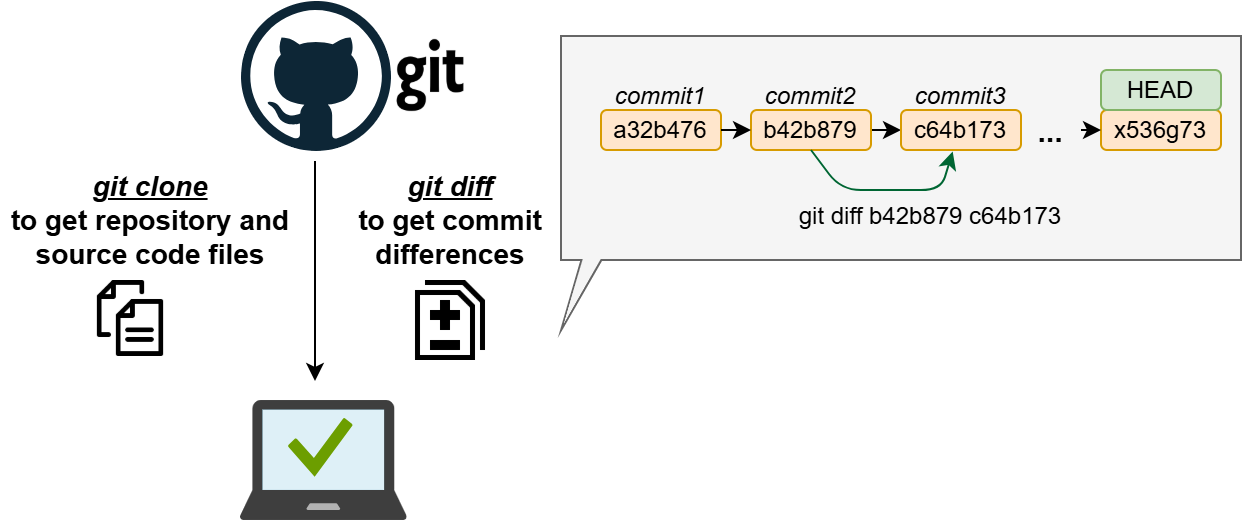
\includegraphics[width=\textwidth]{gitdata.png}
\caption{Using Git commands (\texttt{clone} and \texttt{diff}) to retrieve source code and commit changes.}
\label{fig:extracting_data_with_git}
\end{figure}


Listing \ref{lst:git_diff} provides an example of a \texttt{git diff} output for three files: \texttt{User.java}, \texttt{Calculator.java}, and \texttt{Utils.java}. From the diff output, we can identify the names of the changed files and information about added or deleted lines of code, but not the specific entities (e.g., classes or interfaces) from those files. 

To determine the changed entities, we first extract the structural dependencies of the system and create a mapping between the entities defined in each file and the file. Later, we associate the changed files with their corresponding entities when processing the diff files using this mapping \cite{DepSACI, b4, icstcc-2024, enase19}. 

For instance, in this example, the mapping can reveal that \texttt{User.java} contains the class \texttt{User}, \texttt{Calculator.java} contains the class \texttt{Calculator}, and \texttt{Utils.java} contains the class \texttt{Utils}. Even if Java typically enforces a standardized relationship between file and entity names, this is not always the case for other programming languages, so we need a uniform approach.

Using this mapping, we can say that the commit presented in Listing \ref{lst:git_diff} generates three pairs of co-changed entities: \texttt{Utils-Calculator}, \texttt{Utils-User}, and \texttt{Calculator-User}.

\begin{lstlisting}[language=diff, caption={Example output of \texttt{git diff} between two commits.}, label={lst:git_diff}]
commit 1a2b3c4d5e (HEAD -> main)
Author: Developer <developer@example.com>
Date:   Wed Dec 13 12:34:56 2024 +0000

    Refactored code and added new features.

diff --git a/src/User.java b/src/User.java
index abc1234..def5678 100644
--- a/src/User.java
+++ b/src/User.java
@@ -1,5 +1,6 @@
+    public User(String name) {
+        this.name = name;
+    }

-    public void greet() {
+    public void displayGreeting() {
         System.out.println("Hello, " + name + "!");
     }
 }

diff --git a/src/Calculator.java b/src/Calculator.java
index 9876543..2345678 100644
--- a/src/Calculator.java
+++ b/src/Calculator.java
@@ -5,7 +5,7 @@ 
-    public int subtract(int a, int b) {
+    public int subtractNumbers(int a, int b) {
         return a - b;
     }
 }

diff --git a/src/Utils.java b/src/Utils.java
index 56789ab..789abcd 100644
--- a/src/Utils.java
+++ b/src/Utils.java
@@ -3,7 +3,7 @
-    public static String getCurrentTime() {
+    public static String getFormattedTime() {
         return java.time.LocalTime.now().toString();
     }
 }
\end{lstlisting}




\section{Tool for measuring software dependencies}
\label{subsec:tool_measuring_dependencies}

\hspace{4em}To extract structural and logical dependencies, we developed a tool that takes as input the source code repository URL of a given system and extracts the corresponding software dependencies \cite{DepSACI, enase19}. 

From a workflow perspective, the tool performs three main activities: downloading the necessary data from the repository, extracting structural dependencies from the source code, and identifying and filtering co-changing pairs from the repository's commit history. Figure \ref{fig:figworkflow} illustrates these activities, with each block representing a different step from the process.


To get the source code files and the change history, we first need to know the repository URL from GitHub (GitHub is a Git repository cloud-based hosting service). With the GitHub URL and a series of Git commands, the tool can download all the necessary data for dependencies extraction.


As presented in figure \ref{fig:extracting_data_with_git}, the \textit{"git clone"} command will download a repository, including the source code files. The \textit{"git diff"} command will get the differences between two existing commits in the Git repository. 
The tool gets the Git repository and the source code files by executing the "clone" command. Afterward, it gets all the existing commits within the Git repository. The commits are ordered by date, beginning with the oldest one and ending with the most recent one. The tool executes the "diff" command between each commit and its parent (the previous commit). The "diff" command generates a text file that contains the differences between the two commits: code differences, the number of files changed and changed file names.


The first step involves downloading the source code files and change history. This requires the GitHub repository URL, as GitHub is a cloud-based hosting service for Git repositories. Using this URL and Git commands, the tool downloads all the data necessary for dependency extraction.

\begin{figure}[H]
\centering
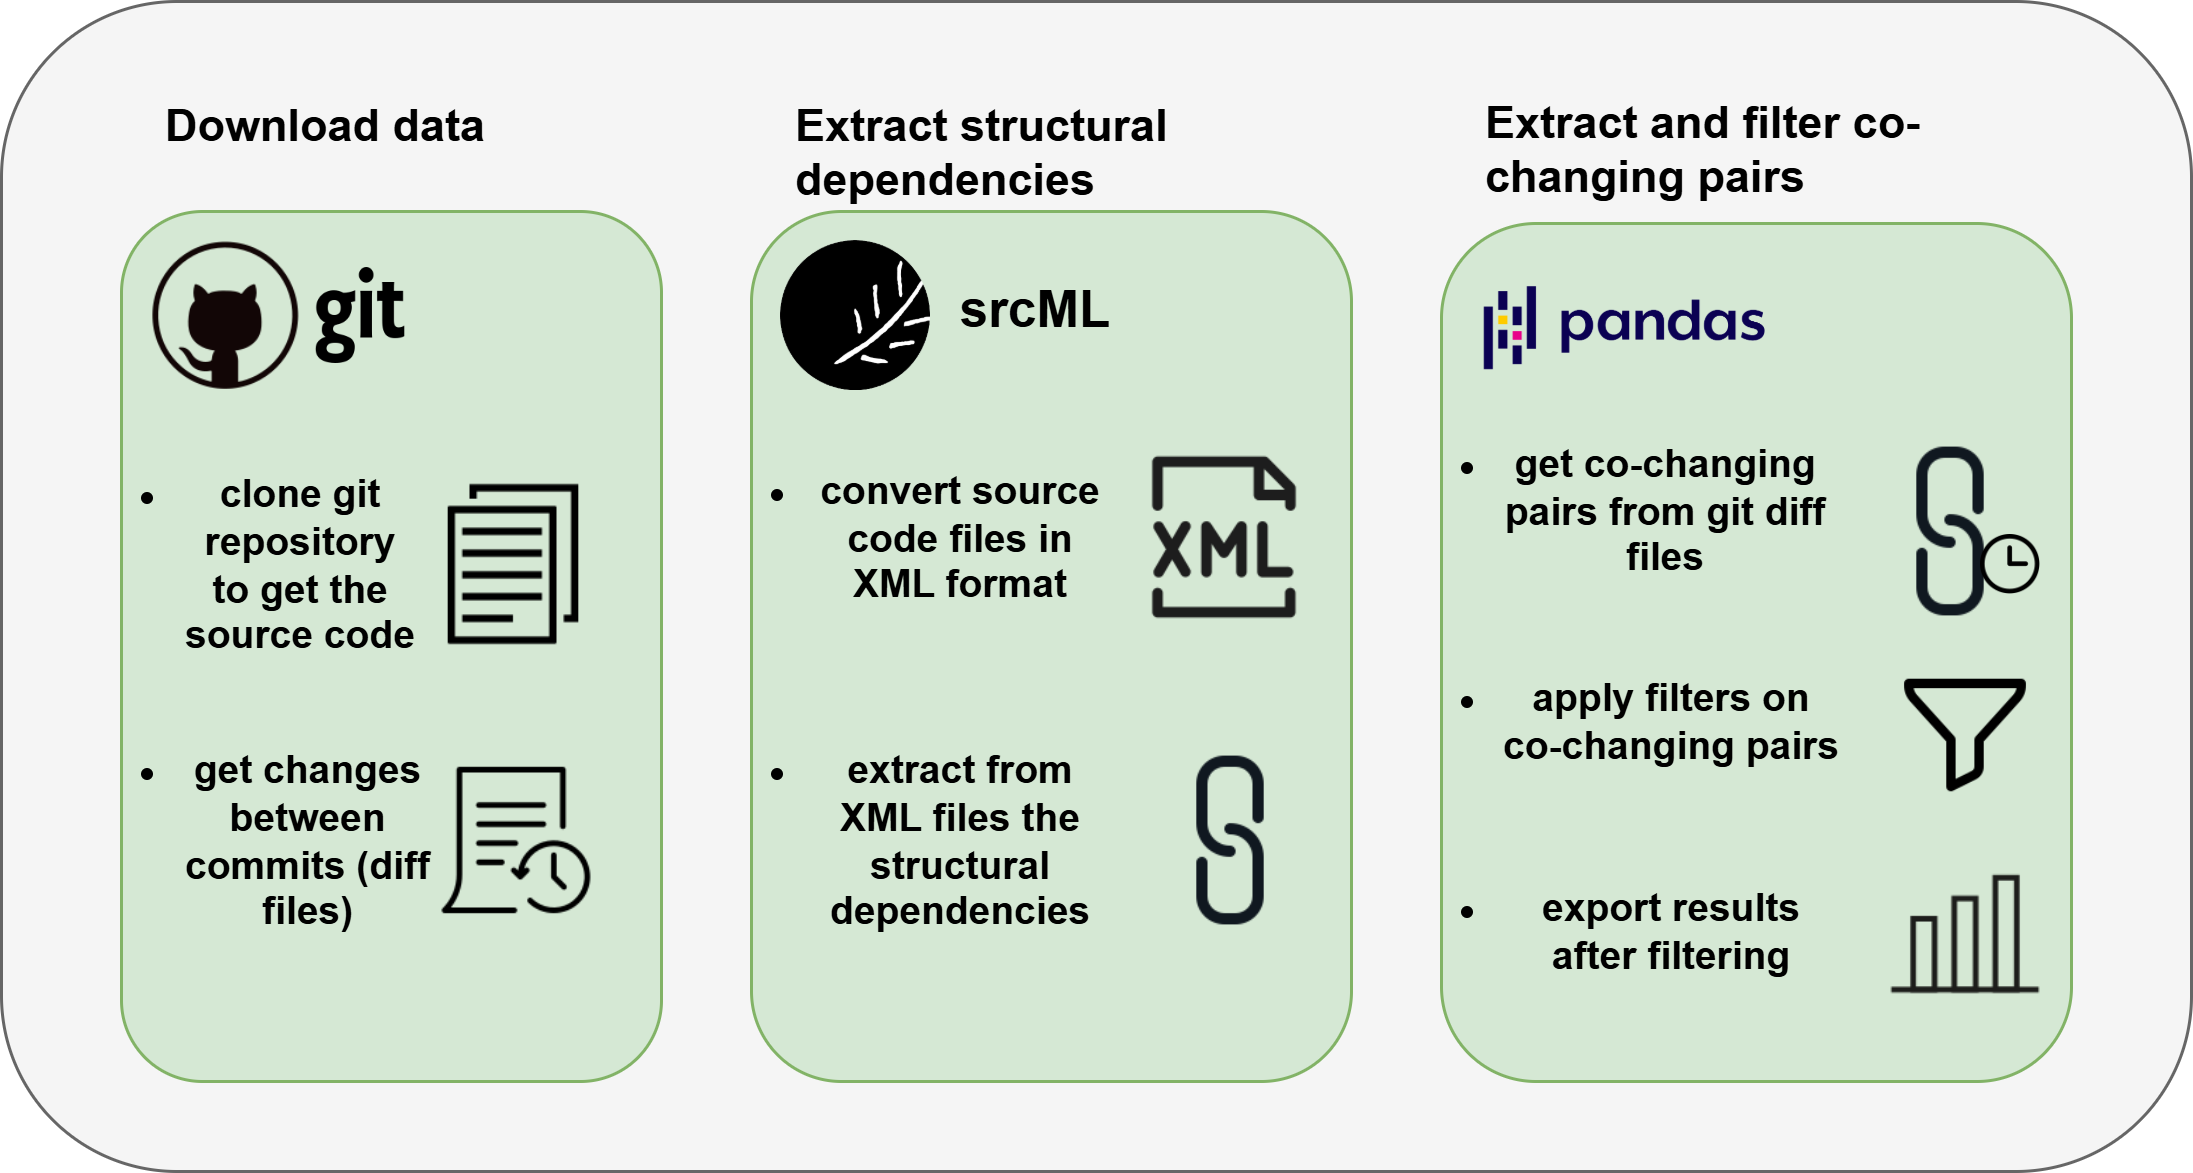
\includegraphics[width=\textwidth]{tool_workflow.png}
\caption{Tool workflow and major activities.}
\label{fig:figworkflow}
\end{figure}



\textbf{Extract structural dependencies.}

To extract structural dependencies from the source code, the tool first converts each source file into the srcML format using the method introduced in subsection \ref{subsec:extracting_structural_dependencies}. The srcML format provides an XML representation of the source code, with markup tags identifying elements of the programming language syntax\cite{srcML}. 

Once converted, the tool parses each file to identify all defined entities (such as classes, interfaces, and enums) from the file. It also detects all entities used by the defined entities. The connections between the defined and used entities form the structural dependencies.


\textbf{Extract and filter co-changing pairs.}

The process of extracting and filtering co-changing pairs is illustrated in Figure \ref{fig:figfiltering}.

To analyze the changes between commits, the tool uses the \texttt{"git diff"} command. All existing commits in the repository are collected and chronologically ordered, starting with the oldest and ending with the most recent. For each commit, the tool runs the \texttt{"git diff"} command to compare it with its parent (the preceding commit). This generates a text file containing the details of the changes between the two commits.

To extract co-changing pairs, the tool parses each generated diff file. From each file, it identifies the number of changed files and their names. Since the tool already knows the software entities contained in each file (from the structural dependencies extraction), it can determine co-changing pairs by linking entities from changed files. Once all the co-changing pairs for a diff file are extracted, the tool moves to the next diff file and repeats the process.

Explained in more detail in subsections \ref{subsec:filtering_transaction_size}, \ref{subsec:filtering_support}, and \ref{subsec:filtering_connection_strength}, not every extracted co-changing pair is considered a logical dependency. For a pair to be considered a logical dependency, it must pass some criteria. These criteria are implemented as filters in the tool. Each filter processes the extracted co-changing pairs and outputs the pairs that meet the filter requirements. The filters can also be combined to ensure that only meaningful logical dependencies remain after filtering.

\begin{figure}[H]
\centering
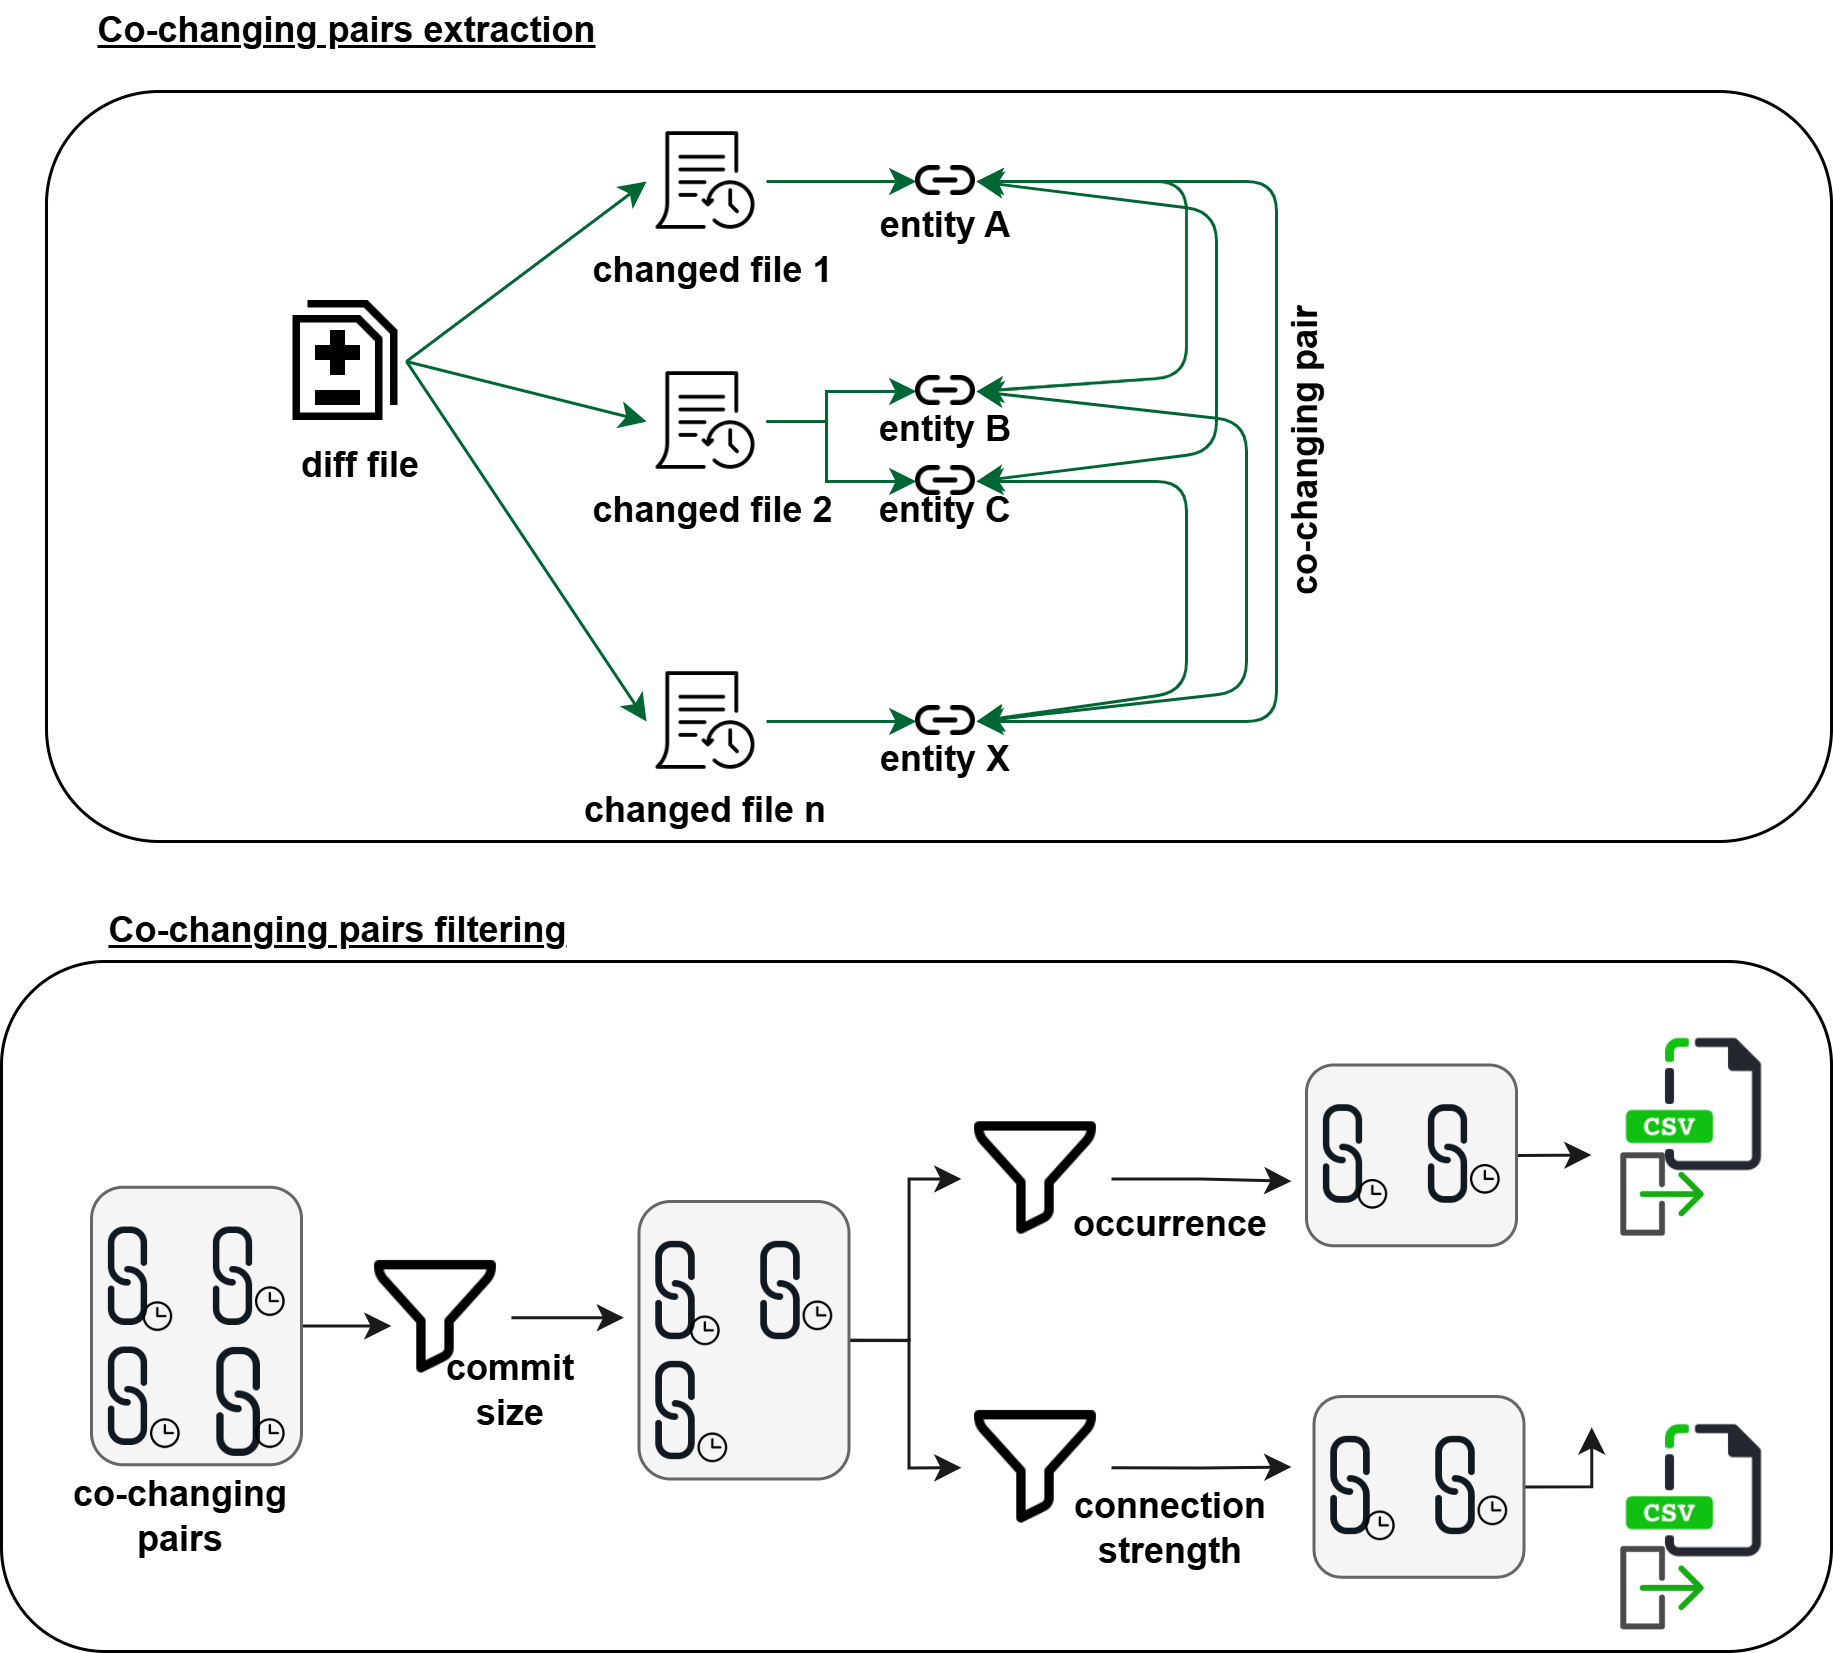
\includegraphics[width=\textwidth]{pairs_filtering.png}
\caption{Co-changing pairs extraction and filtering.}
\label{fig:figfiltering}
\end{figure}



\section{Filtering logical dependencies}
\label{sec:filtering_logical_dependencies}

\hspace{4em}As discussed in Section \ref{ld-intro}, the number of co-changing pairs extracted from software repositories can be quite large, often reaching millions. This quantity, combined with noise in the data, makes it important to apply filtering techniques to identify meaningful co-changing pairs.

This section presents three filtering techniques used to refine the extracted co-changing pairs. The filter based on commit transaction size, discussed in Section \ref{subsec:filtering_transaction_size}, is always applied. The experiments are performed by combining this filter with one of the other two filters: the support filter presented in Section \ref{subsec:filtering_support} or the connection strength filter discussed in Section \ref{subsec:filtering_connection_strength}. The commit size filter aims to reduce the overall size of the co-changing pairs, while the support and connection strength filters aim to minimize noise in the data.

\subsection{Filtering based on commit transaction size}
\label{subsec:filtering_transaction_size}

As discussed in Section \ref{ld-intro}, the number of co-changing pairs extracted from software repositories can be quite large, often reaching millions.  With this filtering approach, the goal is to reduce the total number of extracted co-changing pairs and move closer to identifying meaningful logical dependencies. 

Large commits often involve many files due to non-functional changes like branch merges, folder restructuring, or formatting updates. These types of commits can introduce noise by creating irrelevant co-changing pairs. Dependencies are more meaningful when extracted from commits that involve feature development or bug fixes, where developers modify related code files. However, if multiple unrelated features or fixes are solved into a single commit, it can add false relationships between the entities.

One example of this issue is the initial commit when a system is migrated to a new versioning platform. These commits typically include many files but no functional changes. Another example is merge commits, created automatically during branch integrations. These commits combine changes from multiple smaller commits, which often address different issues or features. In such cases, analyzing the smaller, individual commits provides more accurate information than the overall merge commit \cite{cluster-access}.

Different studies have used various threshold values for filtering commit sizes. Cappiluppi and Ajienka \cite{DBLP:journals/jss/AjienkaC17, DBLP:journals/ese/AjienkaCC18} only considered commits with fewer than 10 modified source code files. Similarly, Kagdi et al. used the same threshold, excluding commits with more than 10 source files. Ying et al. \cite{Ying-co-change} took a different approach, excluding commits involving over 100 files. Zimmermann et al. \cite{Zimmermann:2004:MVH:998675.999460} configured the ROSE tool to exclude commits larger than 30 files. Moonen et al. \cite{Moonen-commit} explored seven different transaction filtering sizes (2, 4, 6, 8, 10, 20, and 30), recommending a threshold of 8 files.



We analyzed the overall transaction size trend for 27 open-source C\# and Java systems with a total of 74,332 commits. The results are presented in Figure \ref{fig:fig_cs} and in Table \ref{table:cs_values}. Based on the analysis, we observed that 90\% of the total commit transactions involved fewer than 10 source code files. This percentage indicates that setting a threshold of 10 files for the maximum size of commit transactions will not affect too much the total number of commits available for extracting co-changing pairs, 90\% of the transactions still remain available for analysis \cite{DepSACI, enase19}.

Table \ref{table:cs_values} provides more details of the commit transaction size distribution for each system. The columns in the table represent the following information:

\hspace{-4em}- \textit{$cs\leq 5$}: The number of commits with a transaction size of 5 or fewer files. \\
- \textit{$cs\leq 10$}: The number of commits with a transaction size of 10 or fewer files. \\
- \textit{$cs\leq 20$}: The number of commits with a transaction size of 20 or fewer files. \\
- \textit{$cs<\infty$}: The total number of commits for the system. \\
- \textit{$Avg$}: The average transaction size for the system.


\begin{figure}[!h]
\centering
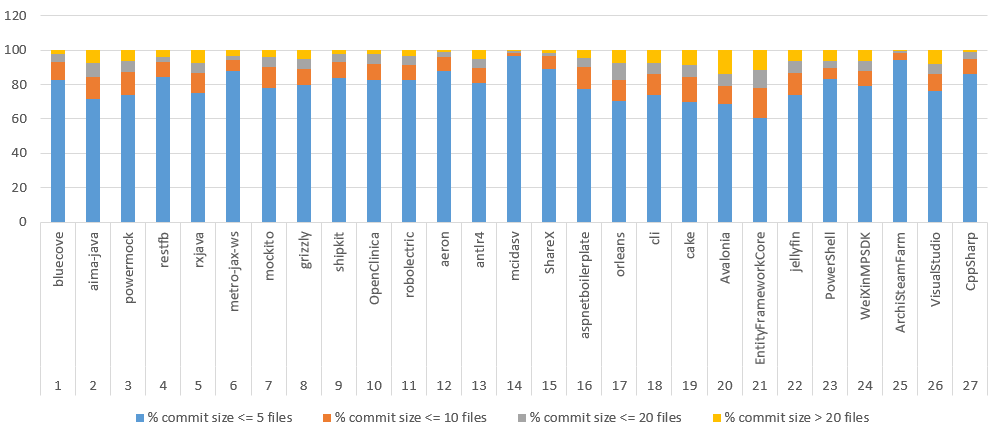
\includegraphics[width=\textwidth]{commit_distribution.png}
\caption{Commit transaction size(cs) trend in percentages.}
\label{fig:fig_cs}
\centering
\end{figure}


\begin{figure}[!h]
\centering
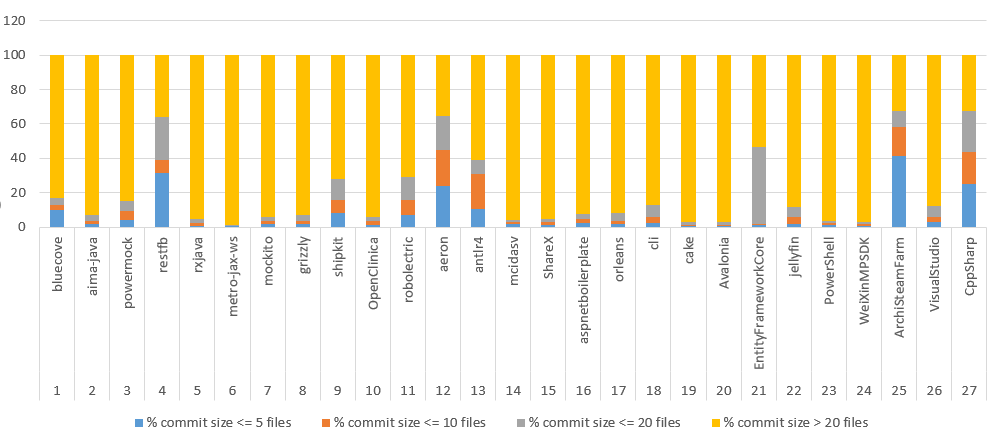
\includegraphics[width=\textwidth]{ld_distribution.png}
\caption{Percentages of co-changing pairs extracted from each commit transaction size(cs) group.}
\label{fig:fig_ld_cs}
\centering
\end{figure}

As we can see in Figure \ref{fig:fig_ld_cs}, even though only 5\% of the commit transactions have more than 20 files changed ($20<cs<\infty$), they generate, on average, 80\% of the total amount of co-changing pairs extracted from the systems.  
The high number of co-changing pairs extracted from such a small number of commit transactions is caused by the number of files involved in those commit transactions.  

One single commit transaction can lead to a large amount of co-changing pairs. For example, in RxJava, we have commit transactions with 1030 source code files. This means that those commits can generate  
\[
\Comb{n}{k}=\frac{n!}{k!(n-k)!} = \frac{1030!}{2!(1028)!} = 529 935
\]
logical dependencies. By setting a threshold on the commit transaction size, we can avoid the introduction of those co-changing pairs into the system.  

Filtering 10\% of the total amount of commit transactions can significantly decrease the number of co-changing pairs. That is why we choose the value of 10 files as our fixed threshold for the maximum size of a commit transaction \cite{DepSACI}.



\begin{table}[!h]
\renewcommand{\arraystretch}{1}
\caption{Commit transaction size(cs) trend and average per system.}
\label{table:cs_values}
\centering
\scalebox{0.9}{
\begin{tabular}{|c|c|c|c|c|c|c|}
\hline
$Nr.$	  & $Project $   &	$cs\leq 5$	&	$cs\leq 10$	&	$cs\leq 20$	&	$cs<\infty$ & Avg	\\ 
\hline
1	&	bluecove	&	738	&	97	&	37	&	22	&	4.9	\\
2	&	aima-java	&	733	&	134	&	74	&	65	&	7.24	\\
3	&	powermock	&	685	&	128	&	66	&	70	&	9.61	\\
4	&	restfb	&	1160	&	127	&	44	&	60	&	9.9	\\
5	&	rxjava	&	3395	&	447	&	253	&	303	&	8.46	\\
6	&	metro-jax-ws	&	2583	&	198	&	78	&	68	&	4.33	\\
7	&	mockito	&	2522	&	433	&	222	&	153	&	6.33	\\
8	&	grizzly	&	2487	&	302	&	180	&	144	&	5.28	\\
9	&	shipkit	&	1311	&	151	&	64	&	37	&	4.26	\\
10	&	OpenClinica	&	2837	&	250	&	119	&	70	&	3.31	\\
11	&	robolectric	&	4827	&	503	&	264	&	318	&	7.43	\\
12	&	aeron	&	4844	&	684	&	300	&	149	&	4.6	\\
13	&	antlr4	&	3426	&	437	&	304	&	264	&	8.5	\\
14	&	mcidasv	&	3996	&	81	&	35	&	24	&	2.47	\\
15	&	ShareX	&	4731	&	529	&	145	&	80	&	4.69	\\
16	&	aspnetboilerplate	&	3208	&	569	&	321	&	225	&	6.61	\\
17	&	orleans	&	2780	&	518	&	369	&	328	&	8.95	\\
18	&	cli	&	3377	&	551	&	308	&	252	&	6.43	\\
19	&	cake	&	1785	&	359	&	174	&	200	&	9.89	\\
20	&	Avalonia	&	3806	&	641	&	371	&	446	&	8.43	\\
21	&	EntityFrameworkCore	&	2866	&	878	&	644	&	822	&	15.38	\\
22	&	jellyfin	&	4007	&	662	&	419	&	345	&	6.25	\\
23	&	PowerShell	&	2702	&	224	&	133	&	191	&	7.33	\\
24	&	WeiXinMPSDK	&	4604	&	526	&	296	&	303	&	9.01	\\
25	&	ArchiSteamFarm	&	2357	&	92	&	28	&	20	&	2.24	\\
26	&	VisualStudio	&	3902	&	521	&	295	&	321	&	6.71	\\
27	&	CppSharp	&	3870	&	390	&	203	&	59	&	3.28	\\
\hline
\end{tabular}
}
\end{table}





\subsection{Filtering based on support}
\label{subsec:filtering_support}

\hspace{4em}In the previous section, we filtered the co-changing pairs based on commit size. Although this reduced the number of extracted co-changing pairs, this type of filtering does not guarantee that the remaining co-changing pairs are valid logical dependencies. A single occurrence of a co-changing pair could represent a valid logical dependency, but it could also be a coincidence.  

To address this, the \textit{support metric} is applied. The support metric of a rule $(A \rightarrow B)$, where $A$ is the antecedent and $B$ is the consequent, is defined as the number of commits (transactions) in which both entities are changed together. Many studies have used the support metric to filter logical dependencies. For example, \textit{Zimmermann et al.} \cite{Zimmermann:2004:MVH:998675.999460} applied minimum support thresholds of 1, 3, and 5 in their ROSE tool, while \textit{Kagdi et al.} \cite{article-Kagdi-commit} used thresholds of 1, 2, 4, and 8.

Considering only co-changing pairs with a minimum support threshold can help improve accuracy. However, for projects with a smaller number of commits, it becomes less likely to find co-changing pairs with high support, which could end up filtering out all the extracted co-changes.

We performed a series of analyses on the test systems, incrementing the support threshold (\textit{support}) from 1 to 4. Co-changing pairs were extracted only from commits with a transaction size of a maximum of 10 files. For each threshold mentioned above, the extracted co-changing pairs were then filtered based on the specified support threshold. Any co-changing pairs that did not meet the minimum support criteria were discarded.


Tables \ref{table:ld_ratio} and \ref{table:sd_percentages} provide detailed results for the support filtering applied to co-changing pairs. Table \ref{table:sd_percentages} presents the percentages of co-changing pairs that are also structural dependencies, and Table \ref{table:ld_ratio} presents the ratio of the number of co-changing pairs to the number of structural dependencies (SD). The columns in the tables represent the following information:

\hspace{-4em}- \textit{$Project\ nr.$}: The unique identifier assigned to each system. \\
- \textit{$support\geq 1$}: Represents the results when the minimum support threshold is set to 1, the ratio of co-changing pairs to structural dependencies (Table \ref{table:ld_ratio}) or the percentage of co-changing pairs that are also structural dependencies (Table \ref{table:sd_percentages}). \\
- \textit{$support\geq 2$}: Represents the results when the minimum support threshold is set to 2. \\
- \textit{$support\geq 3$}: Represents the results when the minimum support threshold is set to 3. \\
- \textit{$support\geq 4$}: Represents the results when the minimum support threshold is set to 4.


\begin{table}[!h]
\renewcommand{\arraystretch}{1}
\caption{Percentage of co-changing pairs that are also structural dependencies.}
\label{table:sd_percentages}
\centering
\scalebox{0.9}{
\begin{tabular}{|c|c|c|c|c|}
\hline
$Project\ nr.$ & $support\geq 1$ & $support\geq 2$ & $support\geq 3$ & $support\geq 4$  \\
\hline
1	&	7,13	&	7,77	&	7,99	&	19,71	\\
2	&	19,54	&	25,76	&	29,55	&	32,16	\\
3	&	6,66	&	8,58	&	11,82	&	14,87	\\
4	&	1,16	&	1,17	&	0,91	&	0,80	\\
5	&	3,99	&	3,96	&	7,75	&	7,49	\\
6	&	13,92	&	20,16	&	22,91	&	22,77	\\
7	&	8,38	&	9,28	&	14,93	&	14,58	\\
8	&	6,70	&	9,73	&	14,20	&	15,60	\\
9	&	16,98	&	23,34	&	29,22	&	32,89	\\
10	&	8,94	&	9,15	&	11,05	&	10,59	\\
11	&	4,99	&	6,92	&	8,88	&	11,08	\\
12	&	13,19	&	17,15	&	18,60	&	19,57	\\
13	&	2,43	&	5,59	&	8,33	&	8,21	\\
14	&	13,27	&	18,88	&	19,02	&	19,28	\\
15	&	12,90	&	21,95	&	25,51	&	27,01	\\
16	&	13,33	&	17,34	&	18,53	&	16,24	\\
17	&	6,09	&	6,18	&	6,41	&	6,44	\\
18	&	9,73	&	10,60	&	14,27	&	18,80	\\
19	&	10,26	&	13,54	&	13,64	&	12,60	\\
20	&	12,83	&	18,36	&	21,00	&	25,72	\\
21	&	2,86	&	4,65	&	5,70	&	4,98	\\
22	&	5,20	&	6,56	&	8,18	&	8,90	\\
23	&	8,23	&	13,64	&	17,04	&	17,65	\\
24	&	6,77	&	10,89	&	14,47	&	16,05	\\
25	&	9,85	&	10,15	&	11,65	&	11,33	\\
26	&	8,65	&	10,79	&	12,78	&	14,34	\\
27	&	7,04	&	8,78	&	9,87	&	10,08	\\
\hline
Avg	&	8,93	&	11,88	&	14,23	&	15,55	\\
\hline
\end{tabular}
}
\end{table}


\begin{table}[!h]
\renewcommand{\arraystretch}{1}
\caption{Ratio of number of co-changing pairs to number of structural dependencies. }
\label{table:ld_ratio}
\centering
\scalebox{0.9}{
\begin{tabular}{|c|c|c|c|c|}
\hline
$Project\ nr.$  & $support\geq 1$ & $support\geq 2$ & $support\geq 3$ & $support\geq 4$  \\
\hline
1	&	4,13	&	1,94	&	1,23	&	0,26	\\
2	&	0,81	&	0,33	&	0,16	&	0,10	\\
3	&	5,12	&	1,93	&	0,78	&	0,38	\\
4	&	53,36	&	42,00	&	38,31	&	36,30	\\
5	&	4,27	&	2,90	&	0,88	&	0,72	\\
6	&	1,07	&	0,46	&	0,30	&	0,23	\\
7	&	4,09	&	2,38	&	0,99	&	0,73	\\
8	&	4,06	&	1,57	&	0,76	&	0,49	\\
9	&	3,64	&	2,03	&	1,14	&	0,77	\\
10	&	1,41	&	1,01	&	0,47	&	0,34	\\
11	&	7,91	&	4,47	&	2,93	&	2,03	\\
12	&	3,92	&	2,15	&	1,47	&	1,07	\\
13	&	10,15	&	3,18	&	1,22	&	1,03	\\
14	&	3,07	&	1,53	&	1,16	&	0,97	\\
15	&	2,34	&	0,84	&	0,48	&	0,33	\\
16	&	1,21	&	0,47	&	0,26	&	0,19	\\
17	&	2,99	&	1,83	&	1,11	&	0,84	\\
18	&	2,26	&	1,37	&	0,67	&	0,40	\\
19	&	2,32	&	1,38	&	0,76	&	0,67	\\
20	&	1,24	&	0,58	&	0,35	&	0,18	\\
21	&	5,33	&	2,12	&	1,27	&	1,05	\\
22	&	3,38	&	1,88	&	0,99	&	0,74	\\
23	&	3,62	&	1,22	&	0,76	&	0,37	\\
24	&	2,57	&	1,22	&	0,67	&	0,46	\\
25	&	7,47	&	5,36	&	4,16	&	3,73	\\
26	&	4,03	&	2,16	&	1,50	&	1,15	\\
27	&	7,46	&	4,26	&	2,99	&	2,43	\\
\hline
Avg	&	5,67	&	3,43	&	2,51	&	2,15	\\
\hline
\end{tabular}
}
\end{table}
Based on Table \ref{table:sd_percentages}, we observe that only a small percentage of the extracted co-changing pairs overlap with structural dependencies. This observation is consistent with findings from related works \cite{DBLP:journals/jss/AjienkaC17, DBLP:journals/ese/AjienkaCC18}. The percentage of co-changing pairs that are structural dependencies increases as the minimum support threshold rises.

We calculate the overlap between co-changing pairs and structural dependencies not only to understand how many structural dependencies are reflected in the versioning system through co-changing pairs but also to filter out co-changing pairs that are structural dependencies, as they do not provide new information about the system.

We stopped the minimum support threshold at 4 because, as observed in Table \ref{table:ld_ratio}, systems with IDs 2, 6, 10, and 16 show a ratio below 1, indicating that the number of structural dependencies exceeds the number of co-changing pairs. For systems with IDs 4, 11, 25, and 27, increasing the threshold to 4 does not significantly reduce the difference between the number of co-changing pairs and structural dependencies.

Raising the support threshold beyond 4 might cause filtering out all co-changing pairs for some systems. Therefore, while applying a threshold of 4 filters co-changing pairs to identify logical dependencies, the remaining number of co-changing pairs still significantly exceeds the number of structural dependencies for certain systems.






\subsection{Filtering based on connection strength}
\label{subsec:filtering_connection_strength}
In Section \ref{subsec:filtering_transaction_size}, we applied a filtering rule to exclude co-changing pairs extracted from commits involving more than 10 changed files. This decision was based on the results obtained from analyzing the commit size.

In Section \ref{subsec:filtering_support}, we introduced an additional filter based on the support metric of a co-changing pair. This filter was applied after the commit size filter. However, the results highlighted a challenge: using a fixed threshold for filtering may not be effective across systems of varying sizes. A threshold that works well for smaller systems may need to be increased for medium-sized systems and vice versa.

To address this issue, we introduced another filter complementary to the commit size filter described in Section \ref{subsec:filtering_transaction_size}. This new filter focuses on the connection strength of co-changing pairs. A co-changing pair that appears only once in a system's history may be less reliable than one that occurs more frequently \cite{cluster-access}.

Zimmermann et al. proposed the support and confidence metrics to measure the reliability of co-changes \cite{Zimmermann:2004:MVH:998675.999460}.

The \textit{support metric} for a rule $(A \rightarrow B)$, where A is the antecedent, and B is the consequent, is defined as the number of commits (transactions) in which both entities are modified together.

The \textit{confidence metric} of the same rule $(A \rightarrow B)$, as expressed in Equation \eqref{eq:confidence}, measures the proportion of commits involving both entities relative to the total number of commits where A appears.

\begin{equation}
\text{Confidence}(A \rightarrow B) = \frac{\text{Nr. of commits containing } A \text{ and } B}{\text{Nr. of commits containing } A}
\label{eq:confidence}
\end{equation}


The confidence metric focuses on entities that are modified less frequently but consistently together, rather than entities that are modified more often but with multiple other entities.

For example, assuming that entity \( A \) was changed in 10 commits and, of these 10 commits, 9 also included changes to entity \( B \), the confidence for the rule \( (A \rightarrow B) \) would be 0.9. On the other hand, if entity \( C \) was changed in 100 commits and, of these 100 commits, 50 also included changes to entity \( D \), the confidence for the rule \( (C \rightarrow D) \) would be 0.5 \cite{cluster-access}. This means we would have more confidence in the first pair \( (A \rightarrow B) \) than in the second pair \( (C \rightarrow D) \), even though the second pair has more than five times the number of updates together.


This observation was also made by \textit{Ying et al.} \cite{Ying-co-change}, who analyzed co-change patterns to recommend potentially relevant source code to developers during development tasks. In their study, they did not use the confidence metric, as they considered it misleading when some files are changed much more frequently than others. Instead, they used only support thresholds from 5 to 30.
 

To favor entities that frequently appear in commits together, we calculated a \textit{system factor}. This factor represents the average support metric value for all entity pairs within the system \cite{cluster-access}.

The system factor is then incorporated into the confidence metric calculation by multiplying the two values. To ensure the metric can also serve as a weight alongside structural dependency weights, we scale the resulting value by 100 to make it supraunitary and limit the range between 0 and 100.

This modified formula is referred to as the strength metric, which is defined in Equation \eqref{eq:strength}.

\begin{equation}
\text{strength}(A \rightarrow B) = \text{confidence}(A \rightarrow B) \times 100 \times \text{system factor}
\label{eq:strength}
\end{equation}



\begin{table}[!h]
\renewcommand{\arraystretch}{1}
\caption{Ratio of number of filtered co-changing pairs to number of SD, when strength A and strength B $\geq threshold \%$}
\label{tab:commitstrengthAND}
\centering
\scalebox{0.8}{
\begin{tabular}{|c|cccccccccc|c|}
\hline
$Project\ nr.$  & $\geq10\%$ & $\geq20\%$ & $\geq30\%$ & $\geq40\%$ & $\geq50\%$ & $\geq60\%$ & $\geq70\%$ & $\geq80\%$ & $\geq90\%$ & $\geq100\%$ \\
\hline
1  & 1.326 & 0.658 & 0.433 & 0.401 & 0.244 & 0.199 & 0.195 & 0.022 & 0.011 & 0.011 \\
2  & 0.266 & 0.137 & 0.070 & 0.044 & 0.036 & 0.019 & 0.005 & 0.004 & 0.003 & 0.003 \\
3  & 0.505 & 0.243 & 0.147 & 0.086 & 0.061 & 0.031 & 0.031 & 0.031 & 0.031 & 0.031 \\
4  & 0.822 & 0.163 & 0.045 & 0.017 & 0.011 & 0.002 & 0.001 & 0.001 & 0.001 & 0.001 \\
5  & 0.234 & 0.119 & 0.054 & 0.037 & 0.034 & 0.018 & 0.013 & 0.011 & 0.007 & 0.007 \\
6  & 0.227 & 0.155 & 0.101 & 0.077 & 0.070 & 0.036 & 0.018 & 0.017 & 0.016 & 0.016 \\
7  & 1.590 & 0.804 & 0.357 & 0.288 & 0.215 & 0.088 & 0.052 & 0.036 & 0.032 & 0.032 \\
8  & 2.073 & 0.293 & 0.170 & 0.111 & 0.093 & 0.050 & 0.039 & 0.034 & 0.021 & 0.007 \\
9  & 1.495 & 0.479 & 0.271 & 0.142 & 0.108 & 0.059 & 0.047 & 0.011 & 0.008 & 0.008 \\
10 & 0.253 & 0.135 & 0.093 & 0.078 & 0.062 & 0.042 & 0.024 & 0.019 & 0.019 & 0.017 \\
11 & 0.114 & 0.086 & 0.064 & 0.037 & 0.027 & 0.025 & 0.001 & 0.000 & 0.000 & 0.000 \\
12 & 0.277 & 0.136 & 0.085 & 0.069 & 0.053 & 0.045 & 0.039 & 0.015 & 0.007 & 0.004 \\
13 & 11.363 & 0.721 & 0.031 & 0.010 & 0.007 & 0.004 & 0.000 & 0.000 & 0.000 & 0.000 \\
14 & 3.225 & 0.805 & 0.660 & 0.533 & 0.493 & 0.454 & 0.386 & 0.356 & 0.005 & 0.005 \\
15 & 6.097 & 0.725 & 0.663 & 0.564 & 0.500 & 0.242 & 0.176 & 0.170 & 0.001 & 0.001 \\
16 & 1.302 & 0.333 & 0.219 & 0.146 & 0.094 & 0.045 & 0.014 & 0.008 & 0.007 & 0.007 \\
17 & 0.816 & 0.640 & 0.551 & 0.503 & 0.496 & 0.196 & 0.159 & 0.152 & 0.142 & 0.142 \\
18 & 1.676 & 0.233 & 0.159 & 0.118 & 0.102 & 0.062 & 0.058 & 0.029 & 0.026 & 0.026 \\
19 & 2.335 & 0.753 & 0.614 & 0.337 & 0.075 & 0.021 & 0.007 & 0.004 & 0.004 & 0.004 \\
20 & 0.846 & 0.117 & 0.098 & 0.018 & 0.013 & 0.002 & 0.001 & 0.001 & 0.001 & 0.001 \\
21 & 3.377 & 1.691 & 1.608 & 1.584 & 1.576 & 1.310 & 0.001 & 0.001 & 0.001 & 0.001 \\
22 & 0.132 & 0.006 & 0.003 & 0.002 & 0.002 & 0.000 & 0.000 & 0.000 & 0.000 & 0.000 \\
23 & 1.732 & 1.299 & 0.158 & 0.053 & 0.007 & 0.001 & 0.000 & 0.000 & 0.000 & 0.000 \\
24 & 3.295 & 0.334 & 0.188 & 0.061 & 0.017 & 0.006 & 0.003 & 0.001 & 0.000 & 0.000 \\
25 & 0.897 & 0.479 & 0.429 & 0.423 & 0.412 & 0.403 & 0.339 & 0.009 & 0.001 & 0.000 \\
26 & 1.281 & 0.090 & 0.053 & 0.028 & 0.020 & 0.013 & 0.006 & 0.001 & 0.001 & 0.001 \\
27 & 99.528 & 1.020 & 0.992 & 0.980 & 0.972 & 0.927 & 0.078 & 0.075 & 0.073 & 0.072 \\
\hline
\end{tabular}
}
\end{table}



\begin{table}[!h]
\renewcommand{\arraystretch}{1}
\caption{Ratio of number of filtered co-changing pairs to number of SD, when strength A or strength B $\geq threshold \%$}
\label{tab:commitstrengthOR}
\centering
\scalebox{0.8}{
\begin{tabular}{|c|cccccccccc|c|}
\hline
$Project\ nr.$ & $\geq10\%$ & $\geq20\%$ & $\geq30\%$ & $\geq40\%$ & $\geq50\%$ & $\geq60\%$ & $\geq70\%$ & $\geq80\%$ & $\geq90\%$ & $\geq100\%$ \\
\hline
1  & 1.312 & 1.181 & 0.700 & 0.599 & 0.419 & 0.235 & 0.219 & 0.046 & 0.045 & 0.045 \\
2  & 0.430 & 0.280 & 0.176 & 0.118 & 0.103 & 0.056 & 0.022 & 0.020 & 0.020 & 0.020 \\
3  & 0.508 & 0.328 & 0.234 & 0.179 & 0.150 & 0.092 & 0.091 & 0.091 & 0.091 & 0.091 \\
4  & 0.662 & 0.336 & 0.122 & 0.067 & 0.059 & 0.016 & 0.015 & 0.015 & 0.015 & 0.015 \\
5  & 0.279 & 0.206 & 0.145 & 0.100 & 0.099 & 0.047 & 0.044 & 0.039 & 0.034 & 0.034 \\
6  & 0.271 & 0.261 & 0.204 & 0.172 & 0.160 & 0.106 & 0.082 & 0.081 & 0.080 & 0.080 \\
7  & 2.481 & 1.521 & 0.904 & 0.623 & 0.411 & 0.199 & 0.128 & 0.107 & 0.101 & 0.101 \\
8  & 1.332 & 0.838 & 0.515 & 0.320 & 0.288 & 0.142 & 0.117 & 0.106 & 0.090 & 0.076 \\
9  & 1.376 & 1.083 & 0.725 & 0.515 & 0.424 & 0.191 & 0.149 & 0.105 & 0.094 & 0.094 \\
10 & 0.830 & 0.434 & 0.314 & 0.256 & 0.217 & 0.130 & 0.093 & 0.082 & 0.080 & 0.072 \\
11 & 0.366 & 0.122 & 0.088 & 0.046 & 0.031 & 0.027 & 0.003 & 0.002 & 0.002 & 0.002 \\
12 & 0.781 & 0.449 & 0.265 & 0.190 & 0.160 & 0.096 & 0.062 & 0.031 & 0.021 & 0.018 \\
13 & 11.363 & 0.798 & 0.055 & 0.022 & 0.011 & 0.007 & 0.002 & 0.002 & 0.002 & 0.002 \\
14 & 1.932 & 1.203 & 0.858 & 0.682 & 0.579 & 0.473 & 0.396 & 0.365 & 0.013 & 0.013 \\
15 & 2.681 & 1.292 & 0.916 & 0.730 & 0.593 & 0.287 & 0.210 & 0.201 & 0.017 & 0.017 \\
16 & 1.055 & 0.759 & 0.493 & 0.364 & 0.273 & 0.130 & 0.067 & 0.050 & 0.046 & 0.046 \\
17 & 1.120 & 0.962 & 0.849 & 0.750 & 0.744 & 0.559 & 0.482 & 0.476 & 0.466 & 0.466 \\
18 & 1.676 & 0.762 & 0.560 & 0.434 & 0.375 & 0.269 & 0.237 & 0.149 & 0.142 & 0.142 \\
19 & 1.883 & 1.197 & 1.001 & 0.541 & 0.185 & 0.103 & 0.019 & 0.013 & 0.013 & 0.013 \\
20 & 0.510 & 0.224 & 0.138 & 0.037 & 0.028 & 0.011 & 0.006 & 0.003 & 0.003 & 0.003 \\
21 & 2.636 & 1.888 & 1.695 & 1.623 & 1.608 & 1.317 & 0.006 & 0.006 & 0.006 & 0.006 \\
22 & 0.132 & 0.030 & 0.016 & 0.011 & 0.008 & 0.003 & 0.002 & 0.002 & 0.002 & 0.002 \\
23 & 3.454 & 1.648 & 0.232 & 0.081 & 0.021 & 0.004 & 0.003 & 0.003 & 0.003 & 0.003 \\
24 & 1.342 & 0.603 & 0.327 & 0.144 & 0.080 & 0.047 & 0.015 & 0.008 & 0.007 & 0.007 \\
25 & 5.472 & 1.416 & 0.830 & 0.677 & 0.575 & 0.450 & 0.353 & 0.023 & 0.016 & 0.014 \\
26 & 1.281 & 0.236 & 0.142 & 0.092 & 0.060 & 0.040 & 0.031 & 0.020 & 0.019 & 0.019 \\
27 & 55.038 & 1.343 & 1.106 & 1.044 & 1.030 & 0.983 & 0.449 & 0.443 & 0.441 & 0.439 \\
\hline
\end{tabular}
}
\end{table}

In Table \ref{tab:commitstrengthOR}, the columns represent the ratio between the number of structural dependencies and the number of co-changing pairs that remain after filtering out pairs where at least one factor falls below the specified threshold in the column header.
In Table \ref{tab:commitstrengthAND}, the columns represent the ratio between the number of structural dependencies and the number of co-changing pairs that remain after filtering out pairs where both factors fall below the specified threshold in the column header.

We calculate this ratio between co-changing pairs and structural dependencies to assess the size of the extracted co-changing pairs compared to the structural dependencies in the system. According to surveys \cite{Shtern:2012:CMS:2332427.2332428}, \cite{sar}, the primary reason logical dependencies (i.e., filtered co-changes) are not used together with structural dependencies is their size. Therefore, it is important to evaluate the ratio between the sizes of co-changes and structural dependencies at each filtering step.

The results in Tables \ref{tab:commitstrengthAND} and \ref{tab:commitstrengthOR} show that the number of co-changing pairs is reduced. In most cases, the number of structural dependencies exceeds the number of co-changing pairs after filtering. However, the goal of filtering is not just to reduce the size of co-changing pairs but to ensure that the remaining co-changing pairs truly indicate logical dependencies.

We keep a manageable number of co-changing pairs by filtering out all co-changing pairs that do not co-occur at least 50\% of the time (factor A and factor B $\geq 50\%$). Considering both the output size and the connection strength of these pairs, the remaining co-changing pairs can be regarded as logical dependencies at this stage.

%%%%%%%%%%%%%%%%%%%%%%%%%%%%%%%%%%%%%%%%%%%%%%%%%%%%%%%%%%%%%%%%%%%%%%%%%

\chapter{Combining structural and logical dependencies}
\label{chap:combining_dependencies}


\section{Overlaps between structural and logical dependencies}
\label{sec:dependency_overlaps}

A logical dependency can be also a structural dependency and vice-versa, so studying the overlapping between logical and structural dependencies while filtering is important since the intention is to introduce those logical dependencies among with structural dependencies in architectural reconstruction systems. Current studies have shown a relatively small percentage of overlapping between them with and without any kind of filtering \cite{DBLP:journals/jss/AjienkaC17}. This means that a lot of non related entities update together in the versioning system, the goal here is to establish the factors that determine such a small percentage of overlapping \cite{enase19}.

Since we are first extracting co-changing pairs and only after various filters we call the remaining co-changing pairs logically dependent, we will be studying the overlapping between the remaining co-changing pairs after each filtering stage and the structural dependencies. 
For each system, we extracted the structural dependencies and the co-changing pairs and determined the overlap between the two dependencies sets, in various experimental conditions. 

One variable experimental condition is whether changes located in comments contribute towards logical dependencies. This condition distinguishes between two different cases: 
\begin{itemize}
	\item with comments: a change in source code files is counted as a co-changing pair, even if the change is inside comments in all files
	\item without comments: commits that changed source code files only by editing comments are ignored
\end{itemize}

In all cases, we varied the following threshold values: 
 \begin{itemize}
	\item commit size ($cs$): the maximum size of commit transactions which are accepted to generate co-changes. The values for this threshold were 5, 10, 20 and no threshold (infinity).  
	\item number of occurrences ($occ$): the minimum number of repeated occurrences for a co-change to be counted as logical dependency. The values for this threshold were 1, 2, 3 and 4.  
\end{itemize}

The six tables below present the synthesis of our experiments. 
We have computed the following  values:
\begin{itemize}
	\item the mean ratio of the number of co-changes to the number of structural dependencies (SD)
   	\item the mean percentage of structural dependencies that are also co-changes (calculated from the number of overlaps divided to the number of structural dependencies)	
	\item the mean percentage of co-changes that are also structural dependencies (calculated from the number of overlaps divided to the number of co-changes)
\end{itemize}

In all the six tables, \ref{tab:ratio:comm}, \ref{tab:ratio:nocomm}, \ref{tab:percSD:comm}, \ref{tab:percSD:nocomm},
\ref{tab:percLD:comm}, \ref{tab:percLD:nocomm} we have on columns the values used for the commit size $cs$, while on rows we have the values for the number of occurrences threshold $occ$. The tables contain median values obtained for experiments done under all combinations of the two threshold values, on all test systems. In all tables, the upper right corner corresponds to the most relaxed filtering conditions, while the lower left corner corresponds to the most restrictive filtering conditions.

\begin{table}[!h]
%% increase table row spacing, adjust to taste
\renewcommand{\arraystretch}{1}
\caption{Ratio of number of co-changes to number of SD, case with comments}
\label{tab:ratio:comm}
\centering

\begin{tabular}{|c|c|c|c|c|}
\hline
	      &	$cs\leq 5$	&	$cs\leq 10$	&	$cs\leq 20$	&	$cs<\infty$	\\
\hline
$occ\geq 1$	&	3,39	&	5,67	&	9,00	&	80,31	\\
$occ\geq 2$	&	2,24	&	3,47	&	5,02	&	60,14	\\
$occ\geq 3$	&	1,04	&	2,53	&	3,52	&	44,68	\\
$occ\geq 4$	&	0,90	&	2,16	&	2,88	&	33,47	\\
\hline
\end{tabular}
\end{table}

\begin{table}[!h]
%% increase table row spacing, adjust to taste
\renewcommand{\arraystretch}{1}
\caption{Ratio of number of co-changes to number of SD, case without comments}
\label{tab:ratio:nocomm}
\centering

\begin{tabular}{|c|c|c|c|c|}
\hline
	      &	$cs\leq 5$	&	$cs\leq 10$	&	$cs\leq 20$	&	$cs< \infty$	\\
\hline
$occ\geq 1$	&	3,24	&	5,33	&	7,90	&	67,16	\\
$occ\geq 2$	&	1,35	&	3,27	&	4,72	&	47,39	\\
$occ\geq 3$	&	1,00	&	1,67	&	2,49	&	32,39	\\
$occ\geq 4$	&	0,43	&	1,26	&	1,93	&	22,15	\\
\hline
\end{tabular}
\end{table}

\begin{table}[!h]
%% increase table row spacing, adjust to taste
\renewcommand{\arraystretch}{1}
\caption{Percentage of SD that are also co-changes, case with comments}
\label{tab:percSD:comm}
\centering

\begin{tabular}{|c|c|c|c|c|}
\hline
	      &	$cs\leq 5$	&	$cs\leq 10$	&	$cs\leq 20$	&	$cs< \infty$	\\
\hline
$occ\geq 1$	&	19,75	&	29,86	&	39,29	&	76,59	\\
$occ\geq 2$	&	12,50	&	20,20	&	27,68	&	66,11	\\
$occ\geq 3$	&	8,49	&	14,22	&	19,94	&	55,99	\\
$occ\geq 4$	&	6,58	&	10,95	&	15,76	&	47,12	\\
\hline
\end{tabular}
\end{table}

\begin{table}[!h]
%% increase table row spacing, adjust to taste
\renewcommand{\arraystretch}{1}
\caption{Percentage of SD that are also co-changes, case without comments}
\label{tab:percSD:nocomm}
\centering

\begin{tabular}{|c|c|c|c|c|}
\hline
	      &	$cs\leq 5$	&	$cs\leq 10$	&	$cs\leq 20$	&	$cs< \infty$	\\
\hline
$occ\geq 1$	&	18,88	&	28,47	&	37,44	&	71,12	\\
$occ\geq 2$	&	11,87	&	19,03	&	25,93	&	59,58	\\
$occ\geq 3$	&	8,00	&	13,09	&	18,15	&	48,65	\\
$occ\geq 4$	&	5,85	&	9,94	&	14,27	&	39,07	\\
\hline
\end{tabular}
\end{table}

\begin{table}[!h]
%% increase table row spacing, adjust to taste
\renewcommand{\arraystretch}{1}
\caption{Percentage of co-changes that are also SD, case with comments}
\label{tab:percLD:comm}
\centering

\begin{tabular}{|c|c|c|c|c|}
\hline
	      &	$cs\leq 5$	&	$cs\leq 10$	&	$cs\leq 20$	&	$cs< \infty$	\\
\hline
$occ\geq 1$	&	12,02	&	8,86	&	6,72	&	1,79	\\
$occ\geq 2$	&	15,05	&	11,71	&	9,38	&	2,21	\\
$occ\geq 3$	&	17,45	&	13,97	&	11,57	&	2,86	\\
$occ\geq 4$	&	18,96	&	15,28	&	12,94	&	3,67	\\
\hline
\end{tabular}
\end{table}

\begin{table}[!h]
%% increase table row spacing, adjust to taste
\renewcommand{\arraystretch}{1}
\caption{Percentage of co-changes that are also SD, case without comments}
\label{tab:percLD:nocomm}
\centering
\begin{tabular}{|c|c|c|c|c|}
\hline
	      &	$cs\leq 5$	&	$cs\leq 10$	&	$cs\leq 20$	&	$cs< \infty$	\\
\hline
$occ\geq 1$	&	12,05	&	9,02	&	6,98	&	1,93	\\
$occ\geq 2$	&	15,08	&	12,03	&	9,66	&	2,42	\\
$occ\geq 3$	&	17,78	&	14,37	&	12,24	&	3,28	\\
$occ\geq 4$	&	19,22	&	15,59	&	13,30	&	4,21	\\
\hline
\end{tabular}
\end{table}



\begin{table}[!h]
\renewcommand{\arraystretch}{1}
\caption{Percentage of SD that are also co-changing pairs after connection strength filtering. }
\label{tab:percSDstrength}
\centering
\scalebox{0.8}{
\begin{tabular}{|c|cccccccccc|c|}
\hline
Condition &	$\geq10\%$	&	$\geq20\%$		&	$\geq30\%$		&	$\geq40\%$		&	$\geq50\%$		&	$\geq60\%$		&	$\geq70\%$		&	$\geq80\%$		&	$\geq90\%$		&	$\geq100\%$	 \\
\hline
							
factor A and factor B	&	11.20	&	6.80		&	4.44	&	3.25	&	2.58	&	1.74		&	1.16	&	0.57	&	0.35	&	0.33	\\
factor A or factor B	&	15.94	&	11.02	&	7.56	&	5.59		&	4.52	&	2.90	&	2.00	&	1.33	&	1.04	&	1.02	\\
								
\hline
\end{tabular}
}
\end{table}

\begin{table}[!h]
\renewcommand{\arraystretch}{1}
\caption{Percentage of co-changing pairs that are SD after connection strength filtering. }
\label{tab:percLDtrength}
\centering
\scalebox{0.8}{
\begin{tabular}{|c|cccccccccc|c|}
\hline
Condition &	$\geq10\%$	&	$\geq20\%$		&	$\geq30\%$		&	$\geq40\%$		&	$\geq50\%$		&	$\geq60\%$		&	$\geq70\%$		&	$\geq80\%$		&	$\geq90\%$		&	$\geq100\%$	 \\
\hline
factor A and factor B	&	10.95	&	20.61	&	23.73	&	26.75	&	28.57	&	33.31	&	33.43	&	38.34	&	42.52	&	39.41	\\
factor A or factor B		&	12.19	&   16.85	&	19.41	&	20.70	&	21.63	&	22.84	&	21.86	&	23.08	&	24.00	&	22.73	\\						

\hline
\end{tabular}
}
\end{table}

In order to assess the influence of comments, we compare pairwise Tables \ref{tab:ratio:comm} and \ref{tab:ratio:nocomm},  
Tables \ref{tab:percSD:comm} and \ref{tab:percSD:nocomm} and Tables \ref{tab:percLD:comm} and \ref{tab:percLD:nocomm}. 
We observe that, although there are some differences between pairs of measurements done in similar conditions with and without comments, the differences are not significant.

On the other hand, the overlap between structural and co-changes is given by the number of pairs of classes that have both structural and co-change dependencies. We evaluate this overlap as a percentage relative to the number of structural dependencies in Tables \ref{tab:percSD:comm},\ref{tab:percSD:nocomm} and \ref{tab:percSDstrength}, respectively as a percentage relative to the number of co-changes in Tables \ref{tab:percLD:comm},\ref{tab:percLD:nocomm}, \ref{tab:percLDtrength}.

A first observation from Tables \ref{tab:percSD:comm}, \ref{tab:percSD:nocomm}, and \ref{tab:percSDstrength} is that not all pairs of classes with structural dependencies co-change. The biggest value for the percentage of structural dependencies that are also co-changes is 76.5\% obtained in the case when no filterings are done.

From Tables \ref{tab:percLD:comm}, \ref{tab:percLD:nocomm}, and \ref{tab:percLDtrength} we notice that the percentage of co-changes which are also structural is always low to very low. This means that most co-changes are recorded between classes that have no structural dependencies to each other \cite{enase19}.   





\section{Weight Assignment}
\label{sec:weight_assignment}

\subsection{Structural dependencies weights}
\label{subsec:structural_weights}

Structural dependencies are important for understanding the architecture of a software system because they reveal how different modules interact at the code level. In our research, we extract structural dependencies using a tool from our previous work \cite{b4}. This tool analyzes the source code to identify various relationships between software entities and exports them in CSV format.

Structural dependencies do not all have the same level of influence on a software system’s architecture and behavior. For instance, the relationship between a variable and the class that uses it is not the same as the relationship between a class and the interface it implements. To reflect these differences, we assign different weights to each type of dependency.

The dependency types and weights were previously defined in related works on clustering \cite{SoraConti}, \cite{Finding-key-classes}.

Table \ref{tab:structural_weights} shows the weights assigned to different categories of structural dependencies, as proposed in previous works.

\begin{table}[htbp]
\centering
\begin{tabular}{|c|l|}
\hline
\textbf{Weight} & \textbf{Dependency types} \\
\hline
4 & Interface realization \\
3 & Inheritance, parameter, return type, field, cast, type binding \\
2 & Method call, field access, instantiation \\
1 & Local variable \\
\hline
\end{tabular}
\caption{Weights assigned to different structural dependency types. \cite{Finding-key-classes}}
\label{tab:structural_weights}
\end{table}

The weights are assigned based on the following considerations:

\textit{Weight 4 – Interface Realization:} Assigned the highest weight because it signifies a strong architectural relationship. Implementing an interface means classes are expected to provide specific functionalities.

\textit{Weight 3 – Inheritance, Parameter, Return Type, Field, Cast, Type Binding:} These dependencies represent significant connections between entities. They include inheritance relationships and shared data or types, which affect the behavior and properties of entities.

\textit{Weight 2 – Method Call, Field Access, Instantiation:} These indicate interactions between classes but are less impactful than higher weights. They involve using methods or fields of other classes or creating instances. When a method call, field access, or instantiation occurs multiple times between the same pair of entities, the weight is multiplied by the number of occurrences. For example, if Class A calls a method in Class B three times, the assigned weight would be 6 (weight 2 multiplied by 3).

\textit{Weight 1 – Local Variable:} Given the lowest weight, local variables are the most basic level of interaction.






\subsection{Logical dependencies weights}
\label{subsec:logical_weights}


We refer to logical dependencies as the filtered co-changes between software entities. A co-change occurs when two or more software entities are modified together during the same commit in the version control system. Co-changes indicate that these entities are likely directly or indirectly related or dependent on each other.

Co-changes are associated with a degree of uncertainty. Compared to structural dependencies, where a dependency is certain, co-changes are less reliable. For example, if the system was migrated from one version control system to another, the first commit will include all the entities from the system at that point in time. Should we consider all these entities related to one another in this case? This would introduce false dependencies and reduce the likelihood of achieving accurate results when combining them with more reliable types of dependencies.

Even if we address the issue of the first commit, a developer can still resolve multiple unrelated issues in the same commit (even though development processes do not recommend this).

To solve this problem, in our previous works, we refined some filtering methods to ensure that the co-changes that remain after filtering are more reliable and suitable for use with other dependencies or individually \cite{b4}, \cite{DepSACI}, \cite{enase19}. Based on our previous results, the filters we decided to use further in our research are the commit size filter and the strength filter. Both filters are used together, and the result is the set of logical dependencies that we use to generate software clusters.

It is important to note that the strength metric is only used for filtering and is \textit{not considered as a weight} of the dependencies. The \textit{weight assigned to each dependency is the number of commits in which both entities were updated together}.



\section{Integration techniques}
\label{sec:integration_techniques}



\begin{figure}[t!]
  \centering
  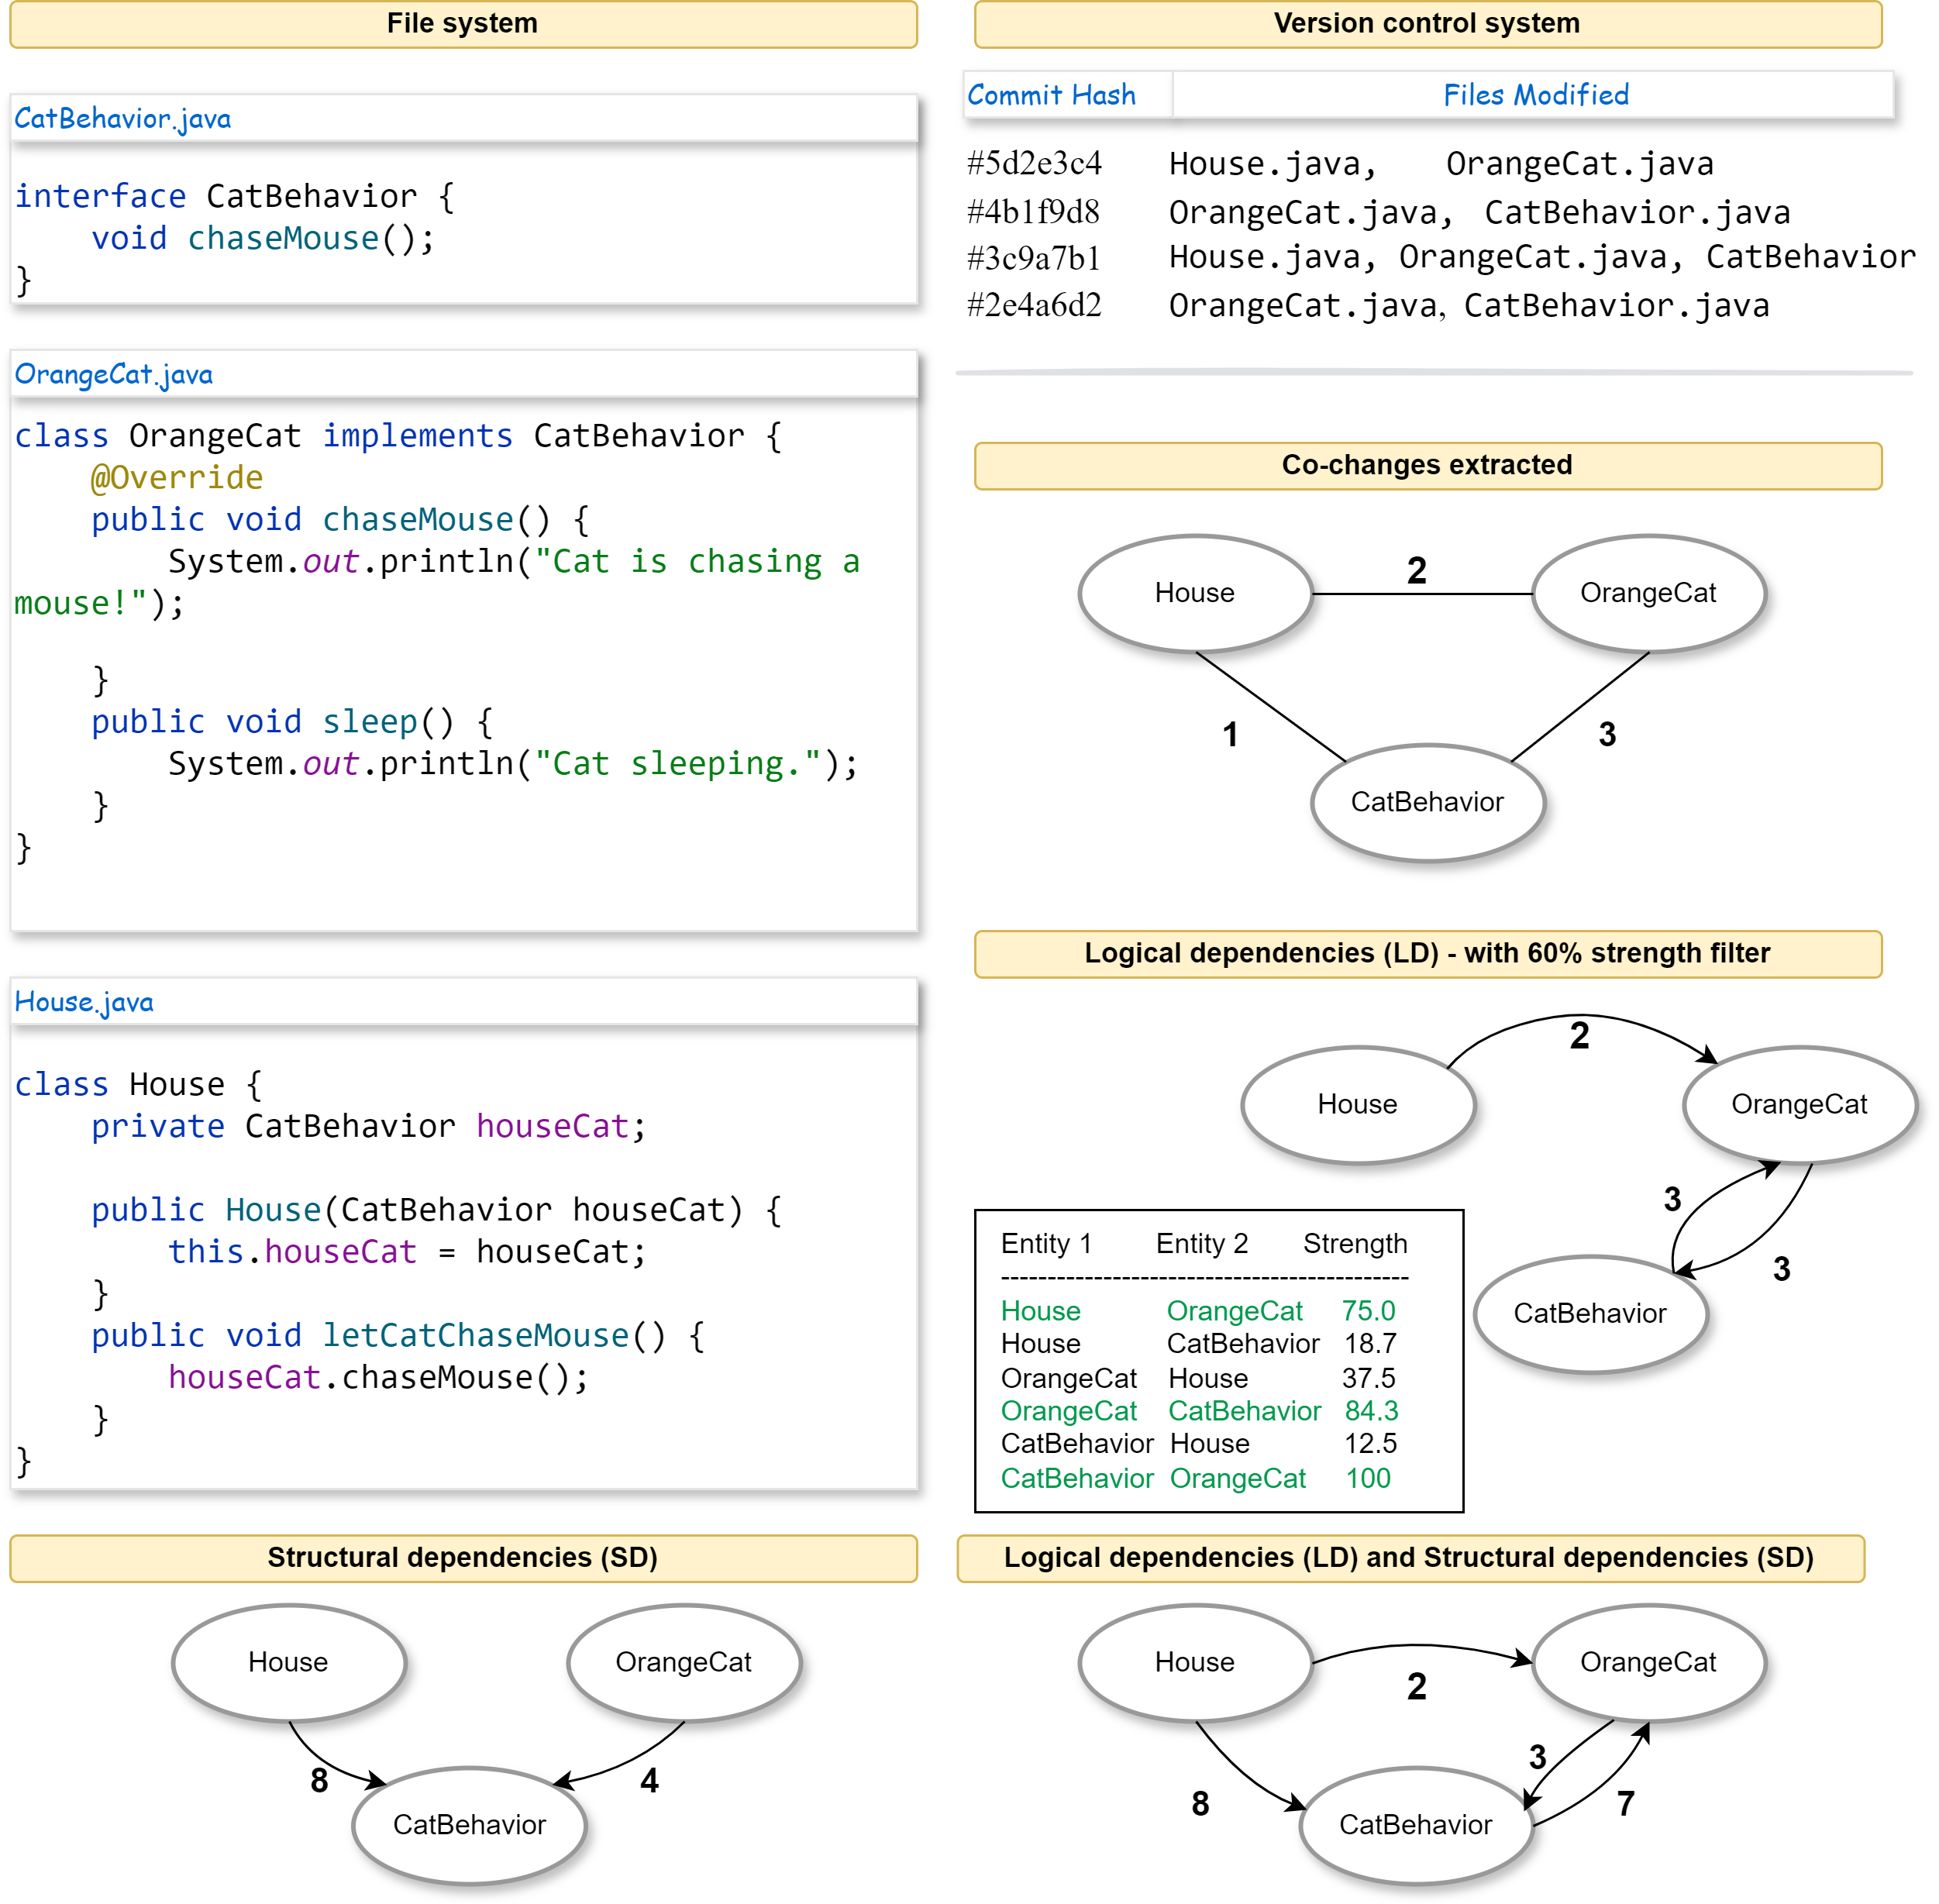
\includegraphics[width=\columnwidth]{codegraph.png}
  \caption{Dependency Graph: Combining structural and logical dependencies.}
  \label{fig:codegraph}
\end{figure}

When structural dependencies (SD) and logical dependencies (LD) are combined in software clustering, both types of relationships are represented within the same graph.

Each entity in the system is represented as a node in the graph, and the dependencies between them are represented as directed weighted edges.

\textit{SD and LD weights are combined} when the same pair of entities appear in both dependencies. In this case, the weights from SD and LD are summed, giving more influence to those entity pairs. When a pair of entities appear only in SD or only in LD, the edge is added to the graph together with its corresponding weight.

Figure \ref{fig:codegraph} illustrates combining structural and logical dependencies in the same dependency graph. The structural dependencies between \texttt{House}, \texttt{OrangeCat}, and \texttt{CatBehavior} entities are visible from the source code analysis.

However, the combination of SD and LD reveals additional insights. One important observation is the logical dependency between \texttt{House} and \texttt{OrangeCat}, which is not observed from the structural analysis. This relation is extracted from version control and filtered using a 60\% strength filter. The strength metric reveals that \texttt{House} and \texttt{OrangeCat} have a significant co-change value of 75.0, usually associated with a strong relationship.

When SD and LD overlap, such as between \texttt{OrangeCat} and \texttt{CatBehavior}, their weights are summed. This summation increases the weight of the dependency, making it more important in the dependency graph.


